\chapter{Metodología}

Con el fin de alcanzar los objetivos planteados en este proyecto de investigación, se reconoce la necesidad de fijar una secuencia y prioridad de actividades. Por ello de se proponen las fases de desarrollo para el proyecto, cada una de las cuales tiene finalidad y funcionalidad dentro del desarrollo del proyecto de investigación. Con fines de realizar control y seguimiento a cada una de las fases, se plantea un cronograma de actividades con intervalos de tiempo conformes a las cargas de trabajo de las actividades a realizar.\\

A continuación se presenta una perspectiva global del proyecto y la descripción de las actividades a desarrollar, para lograr los objetivos propuestos para el proyecto.

%%
	\begin{figure}[ht]
		    \centering
		    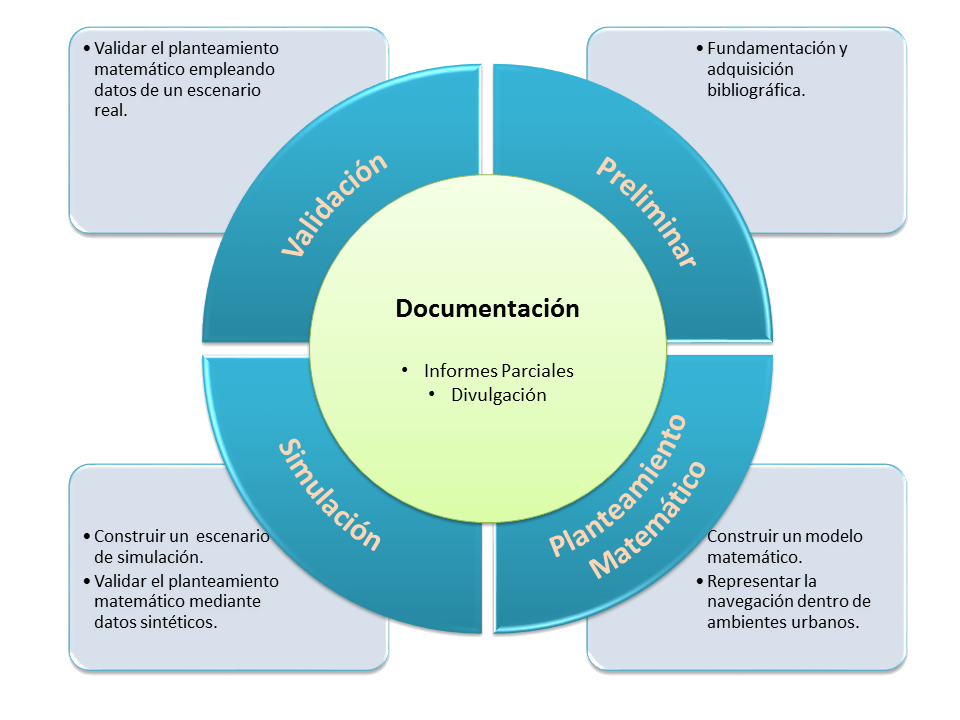
\includegraphics[scale=0.42]{Metodologia.png}
		    \caption{Metodología para el desarrollo del proyecto.}
		    \label{fig:Metodologia}
	\end{figure}


% La metodología a seguir consta de las siguientes fases:

\section{Fundamentación y adquisición bibliográfica}

Durante el transcurso de las cinco (5) semanas iniciales del proyecto (de las 16 destinadas para el desarrollo total); serán destinadas a la contextualización y consulta bibliográfica acerca de sistemas embebidos, procesadores embebidos, modelos de programación y plataformas de cómputo de alto rendimiento; con el fin de tener bases y fundamentos teóricos para enfocar el futuro inmediato del proyecto.\\

Como son el planteamiento del modelo matemático para la técnica de posicionamiento y la selección de un medio de comunicación entre dispositivos para el intercambio de información en materia de observables de posicionamiento.

\section{Construcción del prototipo software}

Esta etapa comprende el desarrollo de una versión simulada de la técnica de posicionamiento, que acoge los planteamientos matemáticos y modelos numéricos considerados necesarios para representar %de la mejor forma 
las condiciones en que se ve involucrado un dispositivo de posicionamiento durante la tarea de posicionamiento dentro de un ambiente urbano.\\

Con el prototipo de software construido se procede a verificar los  resultados numéricos del mismo, con los cuales se tiene un %considerarse como (permiten tener ) 
primer acercamiento al comportamiento y características de la técnica desarrollada; sobre los cuales se puede ejercer criterio y determinar si el planteamiento matemático producto de la fase anterior, es un recurso valido para el alcance del objetivo planteado en la presente propuesta de investigación.

\section{Construcción del prototipo hardware}

Con la ayuda del prototipo de software y los resultados de simulación del planteamiento matemático, se identificará el tipo de información y  medio de comunicación requerido para el intercambio de información entre dispositivos, que permita a la técnica de posicionamiento planteada llevar a cabo el cálculo y solución del posicionamiento del dispositivo que lo emplee.\\

Igualmente se lleva a cabo la integración del software y los  componentes de hardware disponibles, para la creación de receptores GPS con los cuales obtener datos bajo condiciones reales de la técnica de posicionamiento propuesta.

\section{Fase de análisis de caso de estudio}

Con esta actividad se busca clasificar lo datos obtenidos por los receptores GPS al momento de emplear la técnica de posicionamiento propuesta, con el fin de evaluar el nivel de precisión obtenido en escenarios al aire libre y dentro de cañones urbanos.\\

Con base en estos resultados, se busca construir argumentos y conclusiones suficientes para determinar si la técnica de posicionamiento propuesta es una alternativa de solución a la problemática planteada y permite dar respuesta a la pregunta de investigación bajo la cual se origina este trabajo de investigación.

%se pretende hacer un análisis global de la técnica con el fin de identificar deficiencias y mejoras de la misma, que puedan dar paso a trabajos futuros, así también conclusiones


\section{Fase de divulgación}

Durante el desarrollo de cada una de las fases que componen la metodología propuesta, se generan controles de avance del proyecto junto con procesos de redacción y revisiones parciales del documento final; donde se materializa experiencia adquirida y los resultados alcanzados durante cada fase de la investigación.\\

Esta fase de la investigación esta enfocada a la divulgación de los resultados y experiencias adquiridas por medio de una publicación científica; en conformidad a lo definido en el reglamento de general posgrados \footnote{Articulo 114 (numeral c): \textit{En el caso de maestrías de investigación, haber publicado o tener la aprobación para la publicación de un (1) artículo de su autoría, en una revista científica indexada u homologada por Colciencias o con índice de impacto o haber participado con ponencia en, al menos, un (1) evento académico internacional en el campo disciplinar de la maestría.},  Acuerdo 075 de 2013 - Consejo Superior - Univ. Industrial de Santander.},para la obtención del titulo profesional como Magíster en Ingeniería de Sistemas. 